% -*- coding: utf-8 -*-
\documentclass[danish]{beamer}

\usepackage{beamerthemesplit}
\usepackage[utf8]{inputenc}
\usepackage[danish]{babel}

\title{Pentominos\\ \textit{RFID på Afd. J, Århus Sygehus} }
\author{Bent Bisballe Nyeng\\ \textit{deva@aasimon.org} }
\date{24. Juni 2009}
%\date{\today}

\begin{document}

\frame{\titlepage}

\section{Formål}
\subsection{Formål}
\frame{
  \frametitle{Formål}
  \Large
  \begin{center}
    Formålet med projektet er at tilgængeliggøre måledata for
    sundhedspersoner ved minimal arbejdsindsats.
  \end{center}
  \normalsize
}

\subsection{Ønsket procedure}
\frame{
  \frametitle{Ønsket procedure}
  \begin{itemize}
  \item Patient ankommer og bliver registreret.
  \item Patient og operatør sætter sig ved apparatet.
  \item Operatøren foretager måling.
  \item Operatøren og patienten forlader apparatet.
  \item Operatøren og andre sundhedspersoner har med det samme adgang til
    måledataene fra hele afdelingen.
  \end{itemize}
}

\section{Introduktion}
%\section[Oversigt]{}
\frame{
  \begin{center}
    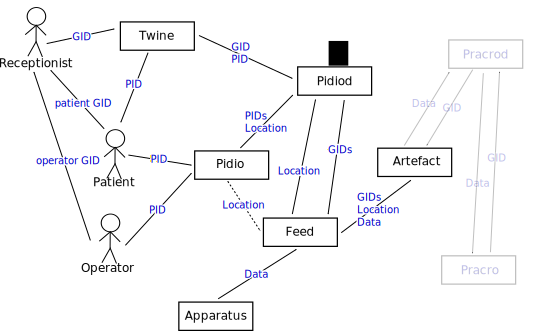
\includegraphics[width=100mm]{overview}
  \end{center}
}

\subsection{Identiteter}
%\section[Oversigt]{}
\frame{
  \begin{center}
    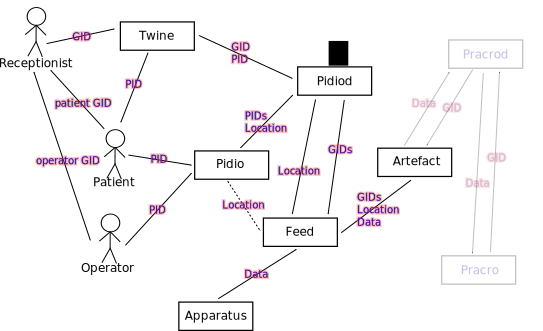
\includegraphics[width=100mm]{overview_ids}
  \end{center}
}

\frame{
  \frametitle{Identiteter}
  \begin{itemize}
  \item Genuine-id (\textit{GID}) er en repræsentation af den faktiske patient
    eller sundhedsperson\\
    (f.eks. cpr nummer).
  \item Pseudo-id (\textit{PID}) er en pseudorepræsentation af et genuine-id\\
    (f.eks. rfid).
  \item Lokation (\textit{Location}) er en symbolsk repræsentation af
    et afgrænset areal med apparater\\(f.eks. et lokalenummer).
  \end{itemize}
  \begin{center}
    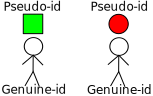
\includegraphics[height=20mm]{pseudo}
  \end{center}
}

\subsection{Servere}
\frame{
  \begin{center}
    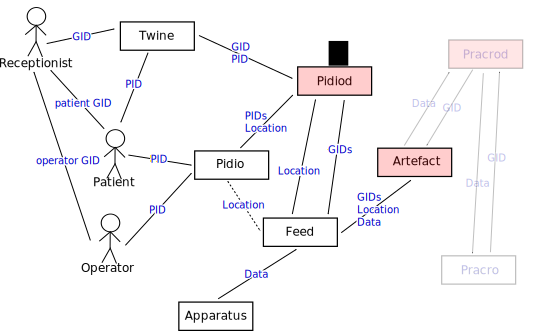
\includegraphics[width=100mm]{overview_servers}
  \end{center}
}

\frame{
  \frametitle{Servere}
  \begin{itemize}
  \item<1-> Pidiod - Identitetsserver, holder styr på sammenkædninger mellem
    GIDer og PIDer.
  \item<2-> Artefact - Dataopsamlingsserver, lagrer data med henblik
    på senere opslag.
  \item<3-> Pracrod - Journalserver, bindeled mellem journalsystemet
    (PC-Praxis) og resten af systemet.
  \end{itemize}
}

\subsection{Klienter}
\frame{
  \begin{center}
    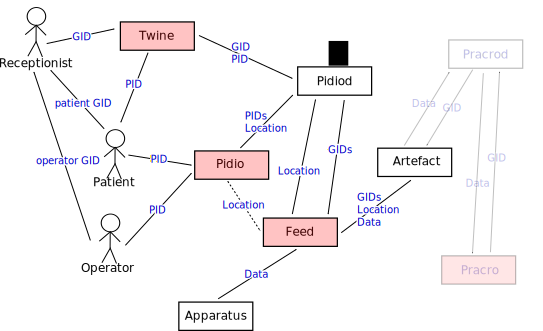
\includegraphics[width=100mm]{overview_clients}
  \end{center}
}

\frame{
  \frametitle{Klienter}
  \begin{itemize}
  \item<1-> Twine - Registreringsklient, bruges ved oprettelse af en
    sammenkædning af et GID og et PID.
  \item<2-> Pidio - Lokation/patient/operatør sammenkobler.
  \item<3-> Feed - Apparat kommunikationsklient, foretager al apparat
    kommunikation og transmitterer data til artefact serveren.
  \item<4-> Pracro - Journalklient.
  \end{itemize}
}

%\section[Oversigt]{}
\frame{
  \begin{center}
    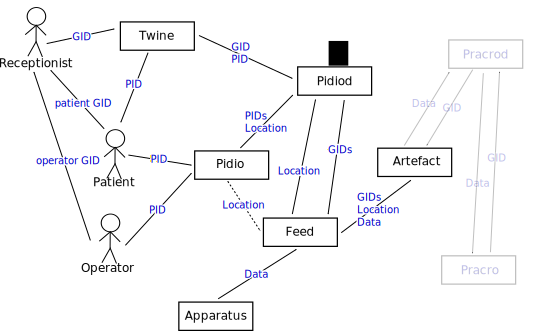
\includegraphics[width=100mm]{overview}
  \end{center}
}

\section{Teknologier}
\subsection{Pseudo-ider}
\frame{
  \frametitle{Pseudo-ider}
  \begin{center}
    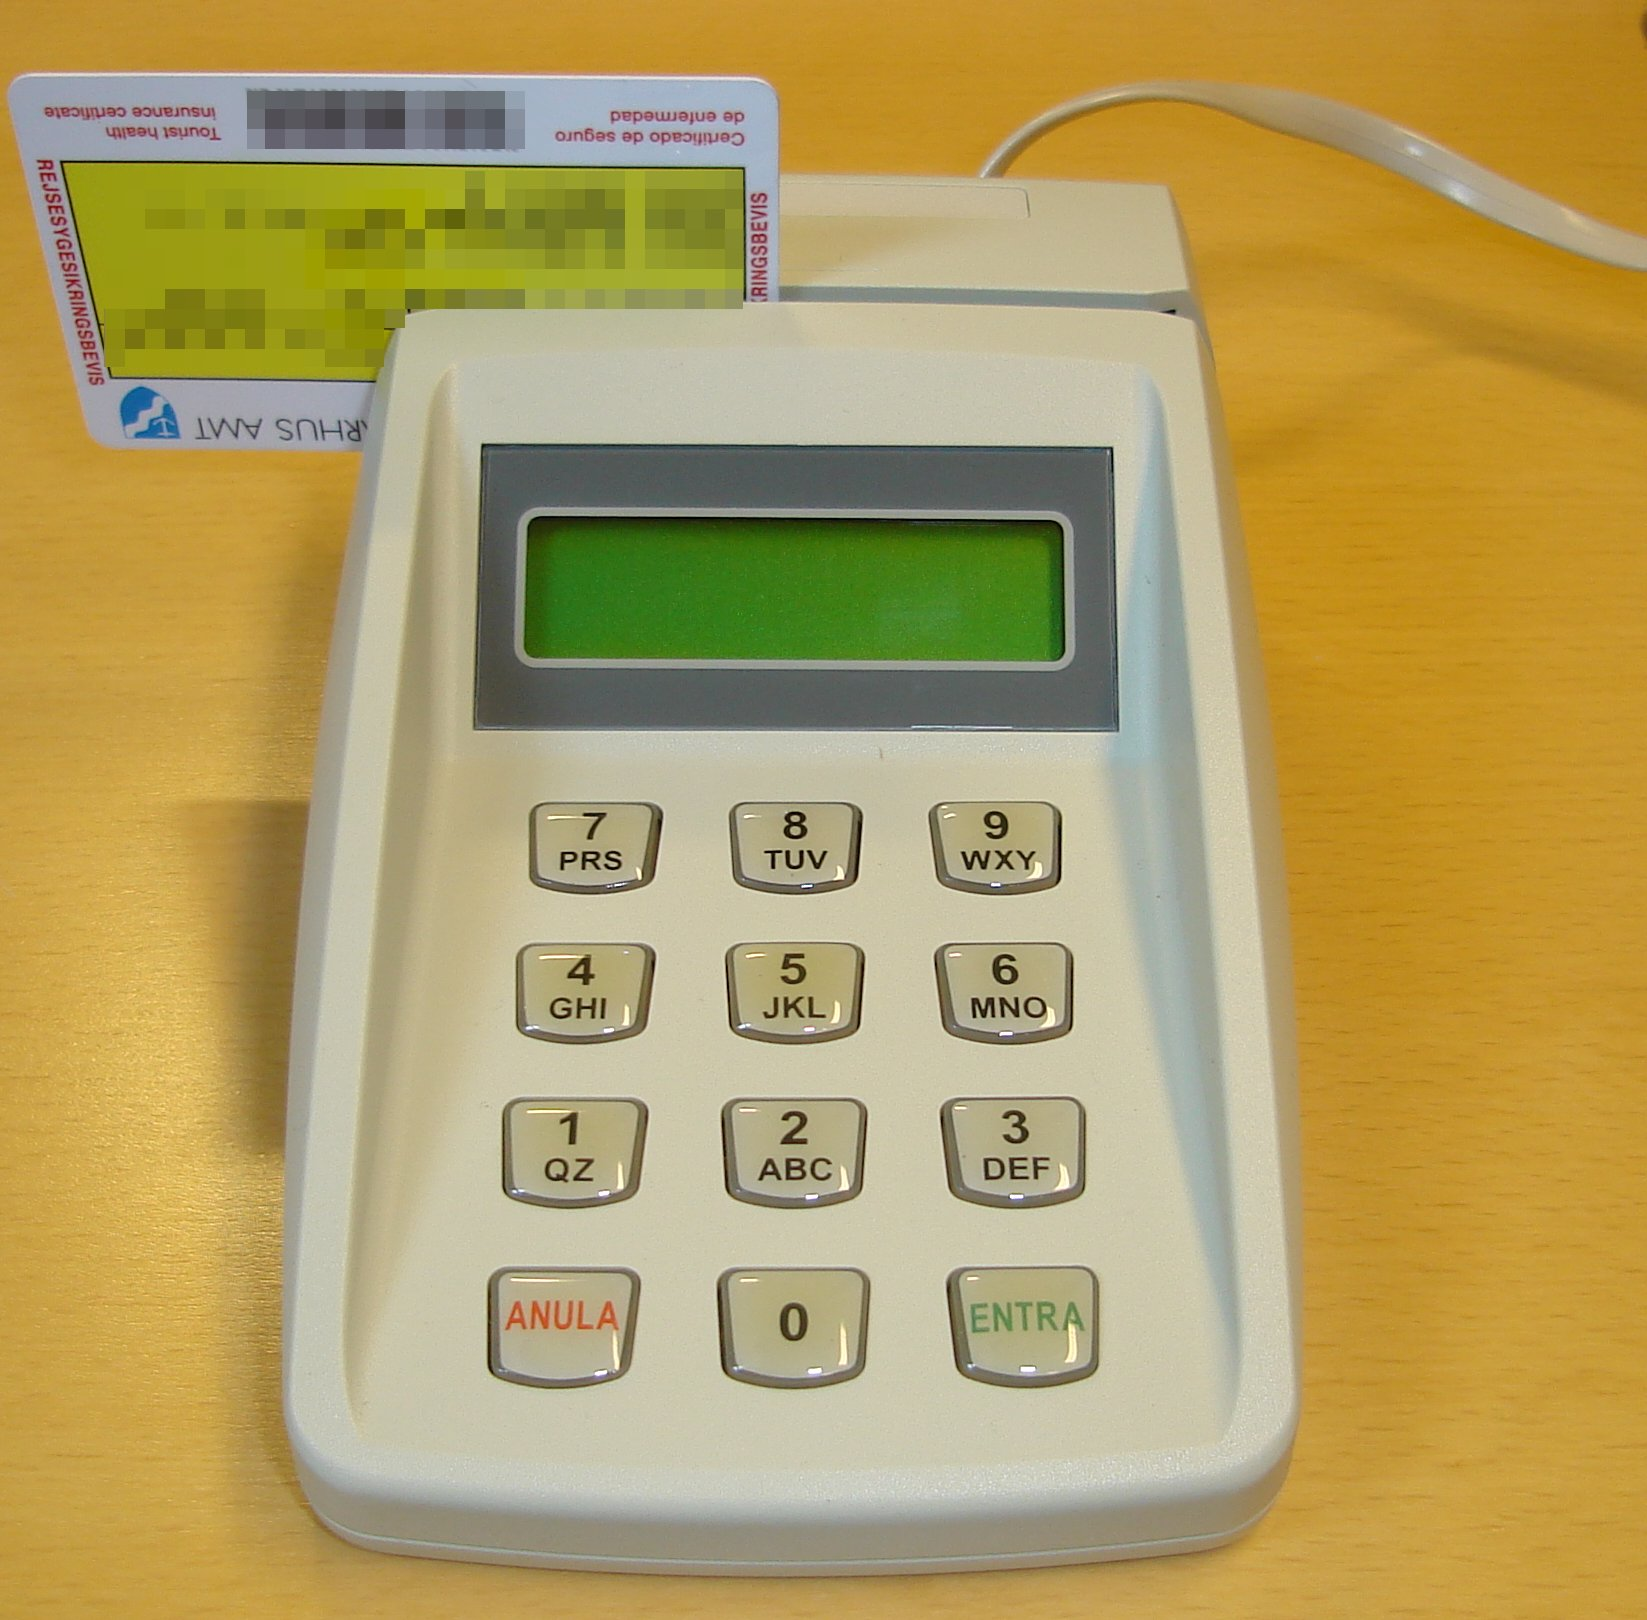
\includegraphics[height=20mm]{../cpr_tastatur}
    \hspace{5mm}
    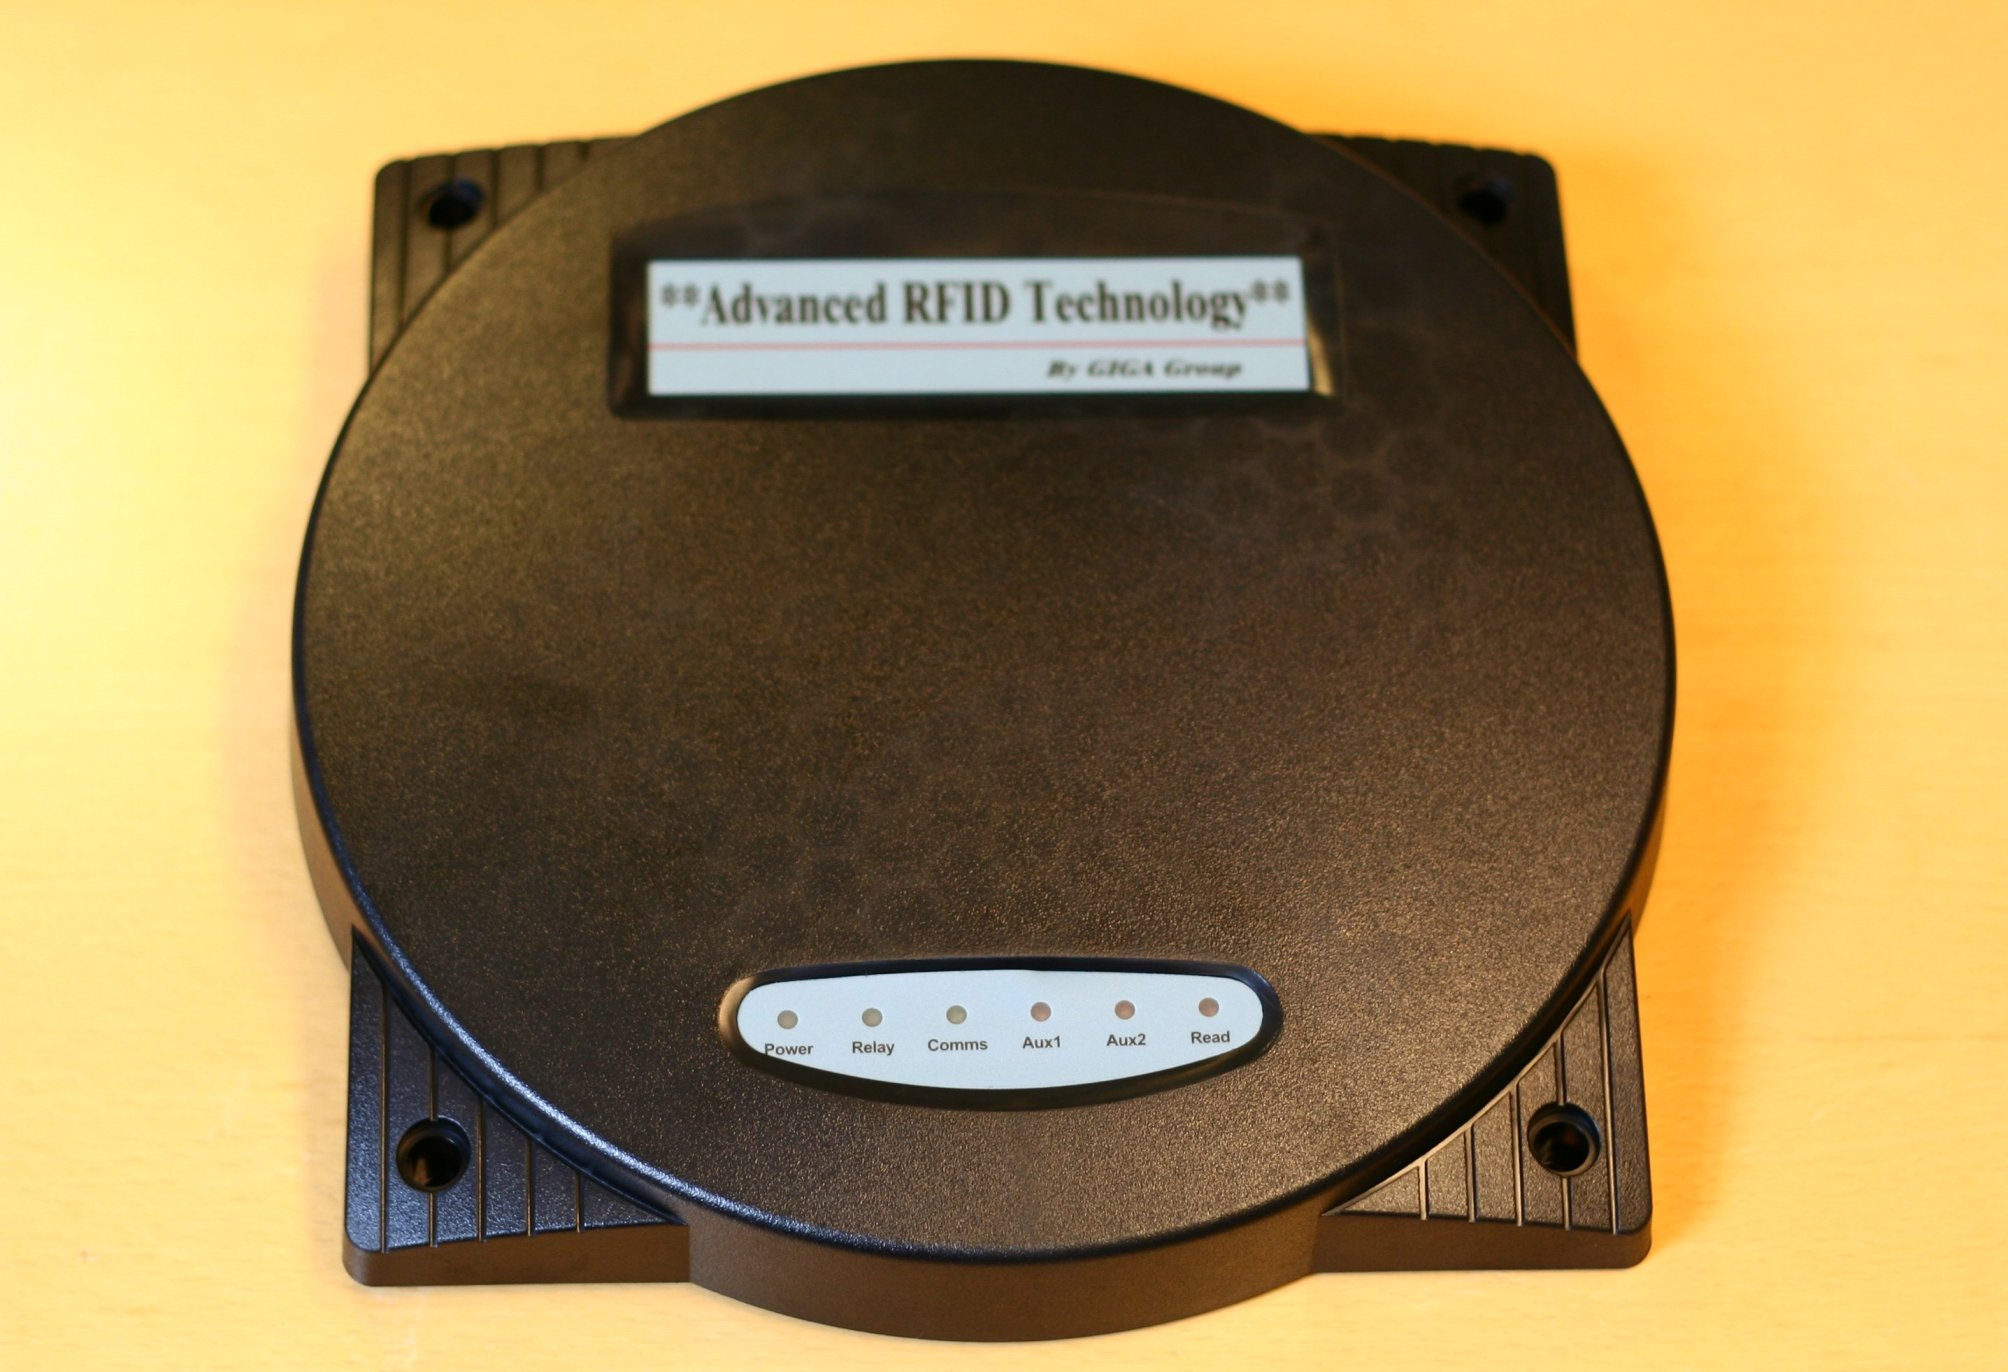
\includegraphics[height=20mm]{../antenne_1}
  \end{center}
  \begin{itemize}
  \item Numerisk tastatur
    \begin{itemize}
    \item Forholdsvis langsom, mulighed for fejlindtastninger.
    \end{itemize}
  \item RFID.
    \begin{itemize}
    \item Langtrækkende (1-2 meter).
    \item Må ikke skabe støj i andet udstyr.
    \item Hurtig, effektiv og fjerner fejlindtastninger
    \end{itemize}
  \end{itemize}
}

\subsection{Protokoller}
\frame{
  \frametitle{Protokoller}
  \begin{itemize}
  \item HTTP lignende protokoller.
  \item XML over TCP/IP til mere komplicerede data transmissioner.
  \end{itemize}
}

\subsection{Datalagring}
\frame{
  \frametitle{Datalagring}
  \begin{itemize}
  \item PostgreSQL (open source database).
  \item Hierarkiske filer på disk.
  \end{itemize}
}

%\subsection{Sikkerhed}
%\frame{
%  \frametitle{Sikkerhed}
%  Løsningen indeholder ingen sikkerhedsmæssige aspekter, og kan derfor
%  f.eks ikke bruges direkte som authentifikation for tilgang til journaldata.
%}

\subsection{Åbenhed}
\frame{
  \frametitle{Åbne teknologier, åbne standarder}
  \begin{itemize}
  \item Al software er udgivet open source (GPL).
  \item Alle protokoller er åbne.
  \item Fleksible systemer som skalerer (kan let udbredes).
  \end{itemize}
}

\section{Demo}
\frame{
  \Huge
  \begin{center}
    Demo
  \end{center}
  \normalsize
}

\end{document}
